\documentclass[../document.tex]{subfiles}
\begin{document}
	
	
	
	
	
	
	\nocite{atkinson2008introduction}
	\nocite{epperson2013introduction}
	Consider an function that is not as smooth as required by Trapeziodal rules. For example if we take $f(x) = \log(1/x)$ to be integrated over interval $[0,1]$ as $f(x)$ is not smooth at $x=0$ and as a result Trapezoid quadrature won't converge to High order. This is because, For optimal via trapezoid rule, we require integrand to be twice continuously differentiable \cite{epperson2013introduction} ,whereas $f(x) = \log(\frac{1}{x})$ doesn't even have first continuous derivative over the interval $[0,1]$.
	
	\begin{simp_num} {\normalfont\textbf{Singularity.}} are points/regions at which an mathematical object is not defined  or takes an infinite value. 
	\end{simp_num}
	
	\begin{simp_num} {\normalfont\textbf{Singular integrand.}} are functions containing singularities in the interval to be integrated, and the specific point at which Singularity integrand does not have value is called 
		{\normalfont\textbf{Points of Singularity}}.
	\end{simp_num}
	
	For instance  $f(x) = \log(\frac{1}{x})$ is a singular functions with 
	$x=0$ as one of its point of Singularity. 
	This chapter focuses on various integration techniques to deal with singular functions.
	%--------------------------------------------
	
	\section{Change of variable}
	Change of variable \cite{atkinson2008introduction} is a prevalent technique to deal with the integral of the form. 
	$$
	I(f) = \int_{a}^{b} f(x)dx
	$$
	Where function $f(x)$ is smooth over the open interval $(a,b)$, but has a Singularity point at one or both endpoints. We can rid of the Singularity by introducing the change of variable i.e
	
	\begin{equation} \label{Change-of-variable}
		x =\phi(t) , \quad \phi(t) = a +\frac{b-a}{\gamma}\Psi(t) ,\quad \Psi(t) =\int_{-1}^{t}\psi(u)du
	\end{equation}
	
	where
	$$
	\psi(t) = \exp \left( \frac{-c}{1 - t^2} \right) \quad \textrm{and} \quad \gamma = \Psi(1)
	$$
	Here, $c>0$ is arbitrary.
	\begin{figure}[h] \label{plot1}
		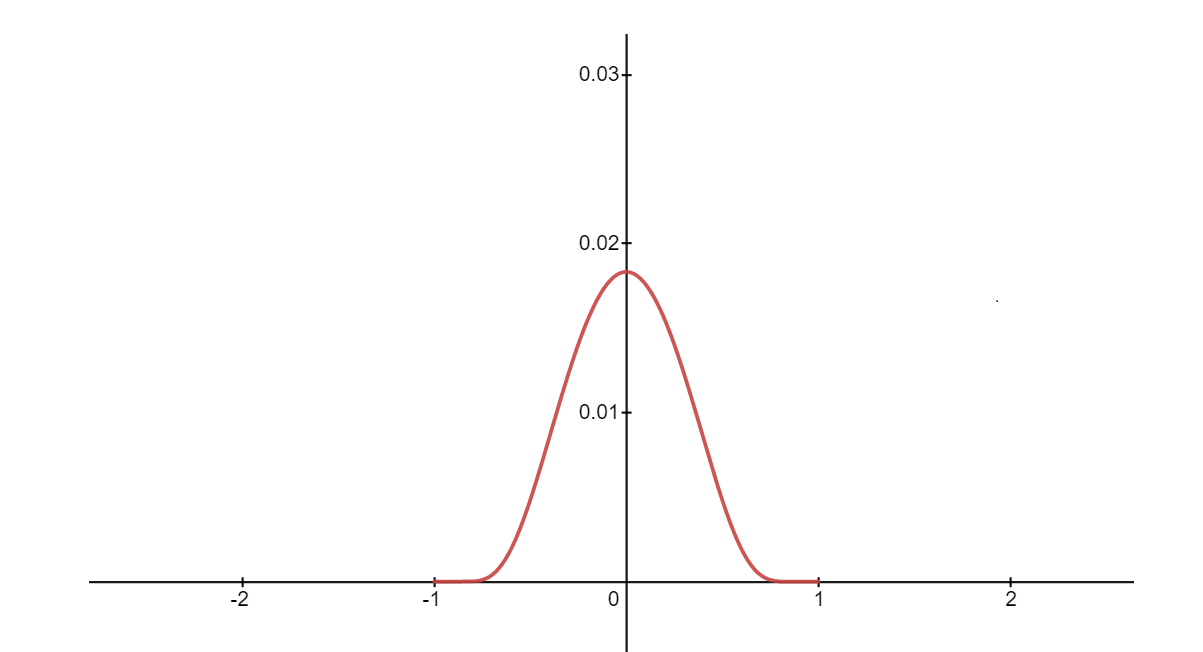
\includegraphics[scale=0.45]{cov_function}
		\centering	
		\begin{center}
			Graph of $\psi(t)$ showing it's behavior as $t\rightarrow \pm1$ over smaller y axis units
			
			\vspace{1mm}
			
			Fig  2.1
		\end{center}
		\caption{Graph of $\psi(t)$ showing it's behavior as $t\rightarrow \pm1$ over smaller y axis units}		
	\end{figure}
	
	\begin{figure}[h] \label{plot2}
		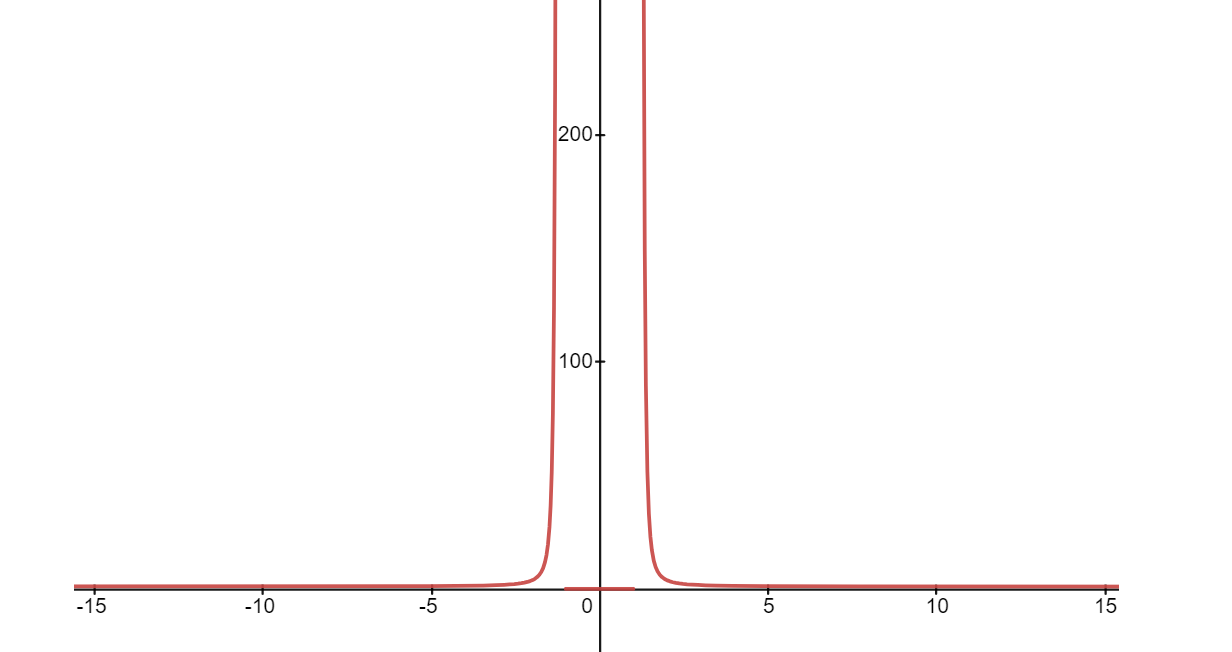
\includegraphics[scale=0.45]{cov_function_l}
		\centering	
		\begin{center}
			Graph of $\psi(t)$ showing it's behavior as $t\rightarrow \pm1$ over larger y axis units
			
			\vspace{1mm}
			
			Fig  2.2
		\end{center}
		\caption{Graph of $\psi(t)$ showing it's behavior as $t\rightarrow \pm1$ over larger y axis units}		
	\end{figure}	
	
	
	Here $\psi$ is constructed to be smooth at $t=\pm1$. 
	As the argument in the exponential goes to $-\infty$ as $t \rightarrow \pm1$ as shown in Fig 2.1 and Fig 2.2. Hence $\psi$ and it's derivatives will vanish at the endpoints. Thus $\psi$ and therefore 
	$\phi $ will be very smooth at endpoints ,which will compensate for almost any non-smooth behavior in $f$. Also change in behavior from $x$ to $t$ will map original interval $[a,b]$ to $[-1,1]$. Now our new integral becomes
	
	\begin{equation}  \label{Change-of-variable-2}
		I(f) = \int_{a}^{b}f(x)dx = \int_{-1}^{1} f(\phi(t)) \phi'(t)dt
	\end{equation}
	
	\begin{examp}
		Take integral of function $f(x) = \sqrt{-log(x)}$ over the interval $[0,1]$.  
		$$
		I(f) = \int_{0}^{1} \sqrt{-log(x)}.dx
		$$
		
		\begin{figure}[h] \label{p2}
			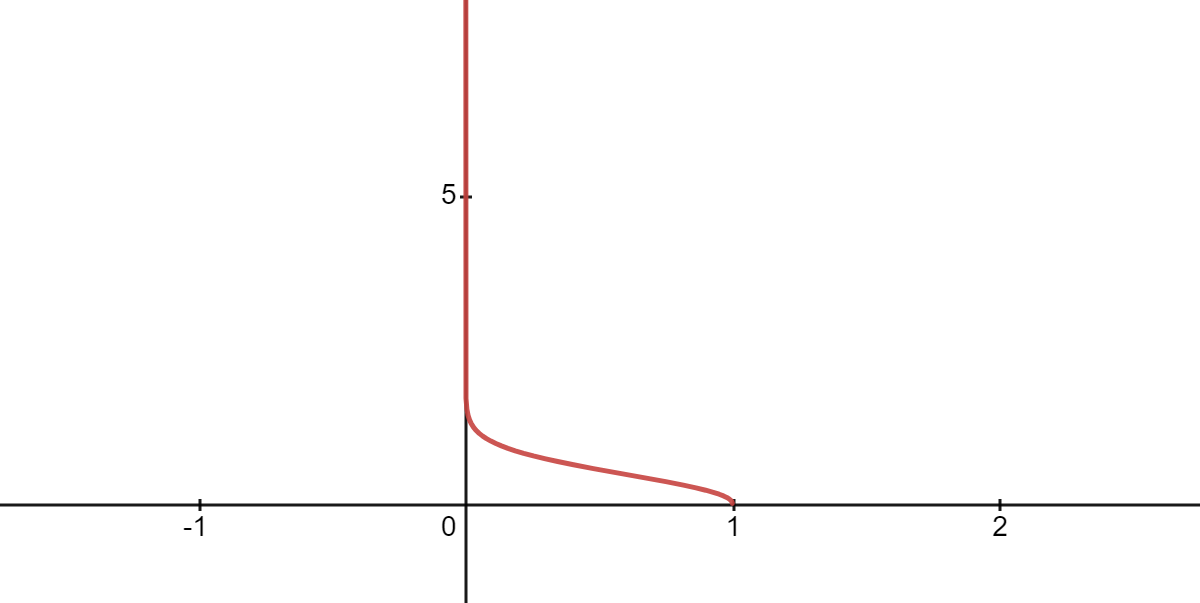
\includegraphics[scale=0.6]{cov_example}
			\centering	
			\caption{Graph of $ \sqrt{-log(x)}$}		
			\begin{center}
				Graph of $ \sqrt{-log(x)}$
				
				\vspace{1mm}
				
				Fig  2.3
			\end{center}
		\end{figure}
		
		
		If we try to approximate its integral by using the n-point Trapezoidal rule.
		
		We do not get any helpful result as $f(x)$ has a singularity at one of its endpoints at $x=0$ as shown in Fig 2.3, and the Trapezoidal rule depends on endpoints. To overcome these problems, one can use the change of variables formula as defined in equation-\ref{Change-of-variable}, and then our integration will change as per equation-\ref{Change-of-variable-2}.
		
		By using change of variables (equation-\ref{Change-of-variable}), our Integral  becomes
		\begin{equation} \label{ex2}
			I(f) = \int_{0}^{1} \sqrt{-log(x)} dx = 
			\int_{-1}^{1}  \sqrt{-log( \phi(t) ) }  \phi'(t)dt
		\end{equation}
		
		If we use the n-point Trapezoidal rule via the change of variables Integral as defined above, then.
		
		%	\addcontentsline{lot}{table}{ 		Error report  of Trapezoidal rule approximation with Change of variables formula for Integral-\eqref{ex2}}
		\begin{table}[h]
			\centering
			\resizebox{\textwidth}{!}{
				\begin{tabular}{ | c || c || c || c| }
					\hline
					N & $\Trapz_n(\sqrt{-log(x)})$  & Error  &Relative Error\\  
					\hline	\hline
					4		&   $8.92023451508737\cdot 10^{-1}$		&	$5.79652605597925\cdot 10^{-3}$ &			 $1.00$	   \\
					8		&	$8.85813283262624\cdot 10^{-1}$		&	$4.13642190133623\cdot 10^{-4}$ &	$7.13\cdot 10^{-2}$\\
					16		&	$8.86218508617344\cdot 10^{-1}$		&	$8.41683541430438\cdot 10^{-6}$ &	$1.45\cdot 10^{-3}$\\
					32		&	$8.86226921208637\cdot 10^{-1}$		&	$4.24412083255277\cdot 10^{-9}$ &	$7.32\cdot 10^{-7}$\\
					64		&	$8.86226930386919\cdot 10^{-1}$		&	$4.93416141278402\cdot 10^{-9}$ &	$8.51\cdot 10^{-7}$\\
					%			128		&	$8.86226930389974\cdot 10^{-1}$		&	$4.93721574734707\cdot 10^{-9}$ &	$8.51\cdot 10^{-7}$\\
					%			256		&	$8.86226930389974\cdot 10^{-1}$		&	$4.93721585836937\cdot 10^{-9}$ & 	$8.51\cdot 10^{-7}$\\
					%			512		&	$8.86226930389974\cdot 10^{-1}$		&	$4.93721563632477\cdot 10^{-9}$ &	$8.51\cdot 10^{-7}$\\
					\hline
					\multicolumn{4}{|c|}{		Table 2.1                 }\\
					\multicolumn{4}{|c|}{Error report  of Trapezoidal rule approximation with Change of variables formula   } \\
					\multicolumn{4}{|c|}{		for Integral-\eqref{ex2}             }\\
					\hline			
			\end{tabular}}
			\caption{ 
				Error report  of Trapezoidal rule approximation with Change of variables formula for Integral-\eqref{ex2}}
		\end{table}
		
		
		
		
		
		
		
		
		
		
		
		Here $N=n-1$, $\Trapz_n(\sqrt{-log(x)})$  is Integral value calculated via (n+1)-point Trapezoidal rule. Error is the absolute difference in values between analytic Integation and Trapezoidal rule approximation $\Trapz_n$.
		We get an approximation of $I(f)$ as required by (n+1)-point Trapezoidal rule by using change of variable formula (equation-\ref{Change-of-variable}).
		
	\end{examp}
	
	%--------------------------------------------
	\section{Analytic treatment of Singularity}
	
	Consider Integral of the form. 
	$$
	I(f) = \int_{a}^{b} f(x)dx
	$$
	divide the interval $[a,b]$ into parts, one containing the singular point and treat it analytically, i.e. if $h \in [a,b]$ is the singular point, then 
	$$
	I(f) =\int_{a}^{b} f(x)dx = \left( \int^{h - \epsilon}_{a} +\int^{h+\epsilon}_{h-\epsilon} + \int^{b}_{h + \epsilon} \right)  f(x)dx
	= I_1 + I_2 + I_3
	$$ 
	where
	$$
	I_1 = \int^{h - \epsilon}_{a} f(x)dx , \quad  I_2 = \int^{h+\epsilon}_{h-\epsilon} f(x)dx \quad \textrm{and} \quad
	I_3 = \int^{b}_{h + \epsilon} f(x)dx
	$$
	we can use any standard quadrature rules on $I_1$ and $I_3$ as $f(x)$ is smooth in 
	$[a,h-\epsilon]$ and $[h+\epsilon,b]$. Coming to $I_2$ , assuming $f(x)$ has a convergent Taylor series, $f(x) = \sum_{j = 0}^{\infty} a_j x^j$. We can evalute
	by replacing $f(x)$ by first few terms of its taylor expansion ,to get fairly accurate results.
	
	
	$$
	I_2 = \int_{h-\epsilon}^{h + \epsilon} f(x)dx 
	= \int_{h-\epsilon}^{h + \epsilon}\sum_{j = 0}^{\infty} a_n x^j dx
	\approx  \int_{h-\epsilon}^{h + \epsilon}\sum_{j = 0}^{k} a_n x^j dx
	$$
	for some $k$ , as 
	$$k\rightarrow \infty \quad \implies \quad
	\int_{h-\epsilon}^{h + \epsilon}\sum_{j = 0}^{k} a_n x^j dx \rightarrow I_2
	$$
	
	\begin{examp} Consider the function $f(x)=cos(x)log(x)$ having singularity at $x=0$ as shown in Fig 2.4, to be integrated over interval $[0,4\pi]$
		
		\begin{figure}[h] \label{coslogx}
			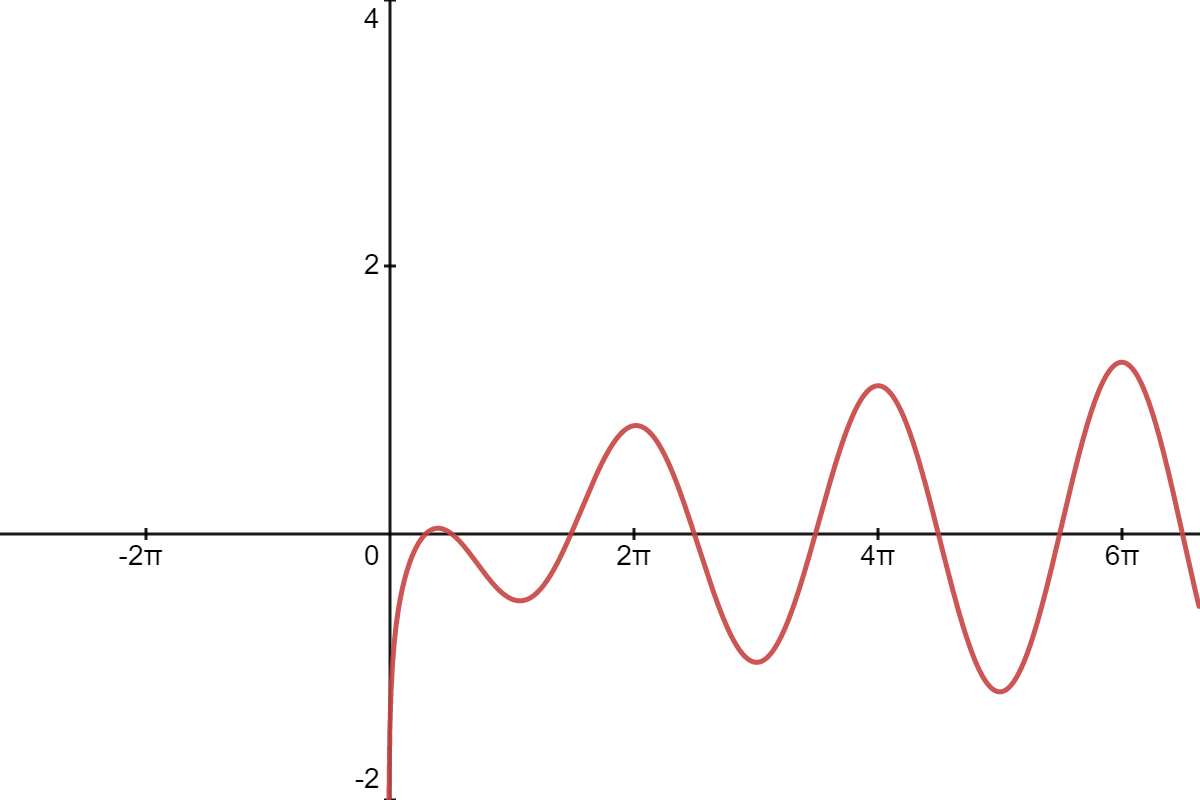
\includegraphics[scale=0.2]{coslogx}
			\centering	
			\caption{Graph of $ cos(x)log(x)$}		
			
			\begin{center}
				Graph of $ cos(x)log(x)$
				
				\vspace{1mm}
				
				Fig  2.4
			\end{center}
		\end{figure}
		\begin{equation*}
			\begin{split}
				\mathcal{I} = \int_{0}^{4\pi} cos(x)log(x)dx  &= 
				\left( \int_{0}^{.1} + \int_{.1}^{4\pi}   \right) cos(x)log(x)dx
				\\ &=  I_1  + I_2
			\end{split}
		\end{equation*}
		
		\begin{equation*}
			\begin{split}
				I_1 &= \int_0^{k}  cos(x)log(x)dx \qquad \qquad  k =0.1\\
				&= k\left[ log(k) - 1 \right]  - \frac{k^3}{6}\left[log(k) - \frac{1}{3} \right] + \frac{k^5}{600}\left[ log(k) - \frac{1}{5} \right] - .... 
			\end{split}
		\end{equation*}
		we can get a very accurate value of $I_1$ by taking the first three terms only. $I_2$  can be calculated by standard quadrature rules or analytically.
		
	\end{examp}
	%--------------------------------------------------------------------------
	%--------------------------------------------------------------------------
	
	%%--------------------------------------------
	\section{Error in Trapezoidal rule}
	
	
	\begin{simp_num}\textbf{\emph{Bernoulli polynomials $\Bernoulli(x)$}} are defined as
		
		\begin{equation}
			\Bernoulli(x) = 
			\sum_{k=0}^{n}  \binom{n}{k} \Bernoulli_{n-k} (x^k)
		\end{equation}
		
		for $n\geqslant0$ with $\mathcal{B}_0(x) =1$ , with properties
		
		\begin{itemize}
			\item $\Bernoulli_1(x) =x - \frac{1}{2}$  ,  
			
			\item $\Bernoulli'(x) =n\Bernoulli_{n-1}(x) $  for $n \geqslant 2$
			
			\item $\Bernoulli(0) =\Bernoulli_n(1) = 0 $ for $n = 3,5,7 ..$
		\end{itemize}
		
		also, Bernoulli polynomials can be generated by a generating function given by Euler, i.e
		$$
		\frac{te^{tx}}{e^t -1} = \sum^{\infty}_{n=0} \Bernoulli_n(x) \frac{t^n}{n!}
		$$
		at $x=0$, it becomes 
		$$
		\frac{t}{e^t -1} = \sum^{\infty}_{n=0} \Bernoulli_n \frac{t^n}{n!}
		$$
	\end{simp_num}
	
	\begin{simp_num}{\normalfont\textbf{Euler-Maclaurin Theorem.}}
		Let $a,b$ with $a<b$ be two real number and let $p\geq1$ be an integer. Then for function $f \in \mathcal{C}_p[a,b]$ ,
		there exist a real number $\xi$ in $(a,b)$ such that
		\begin{equation} \label{euler_macl}
			\int_a^b f(x)dx - \Trapz_n(f) = 
			\sum_{j=1}^{ \lfloor p/2\rfloor -1 }  h^{2j} \frac{\mathcal{B}_{2j}}{2j!}
			\left[
			f^{(2j-1)}(b) - f^{(2j-1)}(a) 
			\right] -  E_n(f) 
		\end{equation}
		$$
		E_n(f) = \frac{h^p  \mathcal{B}_p  }{p!}  f^{ (p)} (\xi)
		$$
		where $\Trapz_n(f)$ is $n+1$ point Trapezoidal rule, $\mathcal{B}_j$ is $jth$ Bernoulli number.
	\end{simp_num}
	
	
	The error of the composite trapezoidal rule ,$ \mathrm{E}_n(f) $ is the difference between the value of the analytical integral and the numerical result via trapezoidal rule.
	\begin{equation*}
		\begin{split}
			\mathrm{E}_n(f) =& \left| \int_a^b f(x)dx - \Trapz_n (f) \right|
			\\
			=& \left| \sum_{j=1}^{ \lfloor p/2\rfloor -1 }  h^{2j} \frac{\mathcal{B}_{2j}}{2j!}
			\left[
			f^{(2j-1)}(b) - f^{(2j-1)}(a) 
			\right] -  \frac{h^p  \mathcal{B}_p  }{p!}  f^{ (p)} (\xi) \right| 
		\end{split}
	\end{equation*}
	
	\begin{lemma}
		Consider a periodic integrand $f \in \mathcal{C}_p[0,T]$ having period $T$. Then $f(0) = f(T)$. Then error in integration of $f$ over interval $[0,T]$ will be given by:
		
		$$
		\mathrm{E}_n(f)
		= \left| \sum_{j=1}^{ \lfloor p/2\rfloor -1 }  h^{2j} \frac{\mathcal{B}_{2j}}{2j!}
		\left[
		f^{(2j-1)}(T) - f^{(2j-1)}(0) 
		\right] -  \frac{h^p  \mathcal{B}_p  }{p!}  f^{ (p)} (\xi) \right|
		$$
		
		A derivative of a periodic function is always periodic with the same period.
		$f(T) = f(0) \implies f^{(j-1)}(T) = f^{(j-1)}(0)$.
		$$
		\mathrm{E}_n(f) = \left| - \frac{h^p  \mathcal{B}_p  }{p!}  f^{ (p)} (\xi)\right| 
		$$
		$$
		\Trapz_n(f) = \int_0^T f(x)dx +  \mathcal{O}(h^p)
		$$
		
		
		
	\end{lemma}
	Trapezoidal rule converges to high order for smooth and periodic functions as illustrated above, whereas, for non-periodic functions approximations, we have to do Endpoints (Boundary) corrections to get high order convergence.
	
	
	%	\textcolor{red}{remark to add why its called endpoint}
	
	%--------------------------------------------------------------------------
	%--------------------------------------------------------------------------	
	%--------------------------------------------------------------------------
	%--------------------------------------------------------------------------	%--------------------------------------------------------------------------
	%--------------------------------------------------------------------------	%--------------------------------------------------------------------------
	%--------------------------------------------------------------------------	
	
	%---------------------------------------------
	%---------------------------------------------
	\section{Endpoints correction}  \label{Endpoints_correction}
	
	Most of the results of this section are taken from \cite{kapur1997high, rokhlin1990end}.
	Before we get to the Endpoint correction, we need the following results for its construction. 
	
	\begin{theorem}[Lagrange Interpolation for Equally-Spaced abscissa] \label{lagrange_uniform}
		
		Suppose $a,b$ are a pair of real number such that $a<b$ , $m \ge 3$ be an integer and $h = \frac{b-a}{m-1}$. 
		
		let $f \in C^{m}[a-mh,b+mh]$ and equispaced points $x_k$ be defined as  $x_k  = \frac{b-a}{2} +kh$.
		Then, for any real number $p$ there exists a real number 
		$\xi , -mh <\xi<mh $, such that
		
		\begin{equation} \label{l11}
			f(x_0 + ph) = \sum_{k} \mathcal{A}_{k}^{m} f(x_k) + \mathcal{R}_{m-1,p}
		\end{equation}
		where $k$ varies from
		
		% \begin{align*}
		%     \frac{1}{2} (m-2) \leq k \leq \frac{1}{2}m &  \quad 
		%     \textit{for even m}\\
		%     \frac{1}{2} (m-1) \leq k \leq \frac{1}{2}(m-1) & \quad 
		%     \textit{for odd m}
		% \end{align*}
		
		
		$$
		-\frac{1}{2}(m-2) \leq k \leq \frac{1}{2}m  \quad 
		\textit{for even m}
		$$
		$$
		-\frac{1}{2}(m-1) \leq k \leq \frac{1}{2}(m-1)  \quad 
		\textit{for odd m}
		$$
		
		with
		$$
		\mathcal{A}_{k}^{m}(p) = 
		\frac{ (-1)^{\frac{m-1}{2}+k} }{
			(\frac{m-1}{2} + k)!
			(\frac{m-1}{2} - k)!
			(p-k)}
		\sum_{t}(p-t)
		$$
		and
		$$
		\mathcal{R}_{m-1,p} = \frac{ h^{m} }{m!} f^{(m)}(\xi)
		\sum_{n} (p-n)
		$$
		here both $t$ and $n$ varies same as $k$. 
	\end{theorem}
	The proof of this theorem can be found in Appendix A.
	
	%---------------------------------------------
	%---------------------------------------------
	
	
	\begin{lemma}
		Let $f;[a,b] \rightarrow \Real$  is a function satisying the conditions of 
		theorem \ref{lagrange_uniform} , and the coefficents $\D_{i,k}^{m}$ are defined as
		
		\begin{equation*}  \label{3coff_initial}
			\D_{i,k}^{m} = 
			\frac{\partial^{2i-1}}{\partial^{2i-1} } \big[
			\mathcal{A}_{k}^{m} (p)
			\big]^{p=0}
		\end{equation*}
		
		where $\mathcal{A}_{k}^{m} (p) ,k,m$ is as same as defined in 
		theorem  \ref{lagrange_uniform} and i is a positive integer.
		
		then
		
		\begin{equation} \label{20}
			f^{(2i-1)} (x_0) = 
			\sum_{k = \frac{-(m-1)}{2} }^{\frac{m-1}{2} } 
			\frac{	\D_{i,k}^{m}   }{	h^{2i-1}	}
			f(x_k) + \BigO(h^m)
		\end{equation}
	\end{lemma}
	
	%---------------------------------------------
	%---------------------------------------------
	
	\begin{theorem}   \label{recussive}
		Suppose $m,l,k$ are integers and coefficients $a^{m}_{k,l}$ are defined by recussive relations
		
		\begin{subequations}  \label{recussive_eqn}
			\begin{align}
				&a^{3}_{1,1} = 1 \label{recussive_eqn_A}   \\
				&a^{3}_{1,2} = 1 \label{recussive_eqn_B}   \\
				&a^{2k+1}_{k,l} = (k - k^2) a^{2k-1}_{k-1,l} + a^{2k-1}_{k-1,l}  + a^{2k-1}_{k-1,l-2}  \label{recussive_eqn_C}   \\
				&a^{m+2}_{k,l} = a^{m}_{k,l-2} -
				\big( \frac{m+1}{2} \big)^2 a^{m}_{k,l} \label{recussive_eqn_D}   
			\end{align}
		\end{subequations}
		
		with $a^{m}_{k,l} = 0$ $\forall$ $k \leq 0 $ or $l \leq 0$ or $m \leq 1$.
		
		then
		$$
		\mathcal{A}_{k}^{m} (p) = 
		\frac{		(-1)^{\frac{m-1}{2} + k}		
		}{	\big( \frac{m-1}{2} +1 \big)!
			\big( \frac{m-1}{2} -1 \big)! 
		}
		\sum_{l=1}^{	\frac{m-1}{2}	}
		a^{m}_{k,l} p^{l}
		$$
		
	\end{theorem}
	
	The following lemma is a corollary of this theorem. 
	%---------------------------------------------
	%---------------------------------------------
	
	\begin{lemma} \label{theorem28}
		Let $m\geq 3$ be an odd integer.Then,
		\begin{equation*}  \label{3coff_final}
			\D_{i,k}^{m} = 
			\frac{		(-1)^{\frac{m-1}{2} + k}		
			}{	\big( \frac{m-1}{2} +1 \big)!
				\big( \frac{m-1}{2} -1 \big)! 
			}
			a_{k,2i-1}^{m} (2i-1)!
		\end{equation*}
		
		for any $k,i$ such that $-\frac{m-1}{2} \geq k \geq \frac{m-1}{2}$, and
		$1 \geq i \geq \frac{m-1}{2}$, with the coefficients $a_{k,l}^{m}$
		defined by the recurrence relation in Lemma \ref{3coff_initial} and $\D_{i,k}^{m}$ from lemma \ref{3coff_initial}.
		
	\end{lemma}
	
	Consider a pair of integers $n,m$ such tha $m\geq3$ and odd ,while $n\geq2$.
	Also let $a\leq b$ be a pair of real numbers , $h = \frac{b-a}{n-1}$ , and 
	$f:[a-mh,b+mh] \rightarrow \Real^{1}$ be an integrable function. Then \emph{Endpoint corrected Trapezoidal rule} $\Trapz_{\alpha^m}^{n}$ 
	( or $\Trapz_{\alpha}^{n}$ ) for nonsingular functions is defined by formula:
	
	\begin{equation}    \label{non_singular_corrected_trapz_rule}
		\Trapz_{\alpha^m}^{n} = \Trapz^{n}(f)  + 
		h \sum_{k = -\frac{m-1}{2}}^{\frac{m-1}{2}} 
		\big(
		f(b+kh) - f(b-kh)
		\big)		\alpha^m_k 
	\end{equation}
	
	where correction coefficients $\alpha^m_k$ is defined as 
	\begin{equation} \label{correction_constants_beta}
		\alpha^m_k = \sum_{l=1}^{\frac{m-1}{2}} 
		\frac{ \D_{i,k}^{m} \Bernoulli_{2l}}{(2l)!}
	\end{equation}
	
	where $\D_{i,k}^{m}$ are defined in $\ref{3coff_initial}$ ( and also $\ref{3coff_final}$ ) and $\Bernoulli_{2l}$ are Bernoulli numbers.
	
	
	\begin{theorem}   \label{righr_end_order_theorem}
		Let $m\geq 3$ and $n\geq 2$ are a pair of integer such that $m$ is an odd integer, then for any $k$ such that 
		$-\frac{m-1}{2} \leq k \leq \frac{m-1}{2}$. Then
		\begin{equation}
			|\alpha^m_k | < 1
		\end{equation}
		where the coefficients $\alpha^m_k$ are defined in \ref{correction_constants_beta}.
		
		Further, suppose $a<b$ be two real number. Then, the Endpoint corrected Trapeziodal rule $\Trapz_{\alpha^m}^{n}$( given by \ref{non_singular_corrected_trapz_rule} ) is of order $m$;i.e , for any 
		$f \in \Cont^m[a-mh,b+mh]$, there exists $c>0$ such that 
		
		\begin{equation}
			\Big|
			\Trapz_{\alpha^m}^{n}(f) - \int_{a}^{b} f(x)dx
			\Big|
			< \frac{c}{ n^{m+1} }
		\end{equation} 
	\end{theorem}
	
	The proofs of theorems \ref{recussive} and \ref{righr_end_order_theorem} can be found Appendix A.
	
	
	
	%--------------------------------------------------------------------------
	%--------------------------------------------------------------------------
	%--------------------------------------------------------------------------
	%--------------------------------------------------------------------------	%--------------------------------------------------------------------------
	%--------------------------------------------------------------------------	%--------------------------------------------------------------------------
	%--------------------------------------------------------------------------	%--------------------------------------------------------------------------
	%--------------------------------------------------------------------------	
	\section{Correction for singular functions}
	
	Suppose a $\Cont^{\infty}$ function $g:(0,1]\rightarrow R$ , defined as
	\begin{equation} \label{singular_func_anguliar}
		g(x) = 	\tau(x)s(x) + \upsilon(x)
	\end{equation}
	where $\upsilon(x) , \tau(x) \in \Cont^k[a,b]$ ,$k \geq 1$ and 
	$s(x) \in \Cont(0, 1]$ an integrable function with a singularity at zero.
	
	
	Consider real numbers $a,b$ such that $a<0$ and $b>0$. Then, Trapeziodal rule can't be used to approximate functions like $g(x)$ over interval $[a,b]$. As $g(x)$ has singularity at $0$ and depending on number of quadrature points taken, we may not get approximations.
	\vspace{3mm}
	
	For example consider $ \int_{-\pi}^{\pi} e^{2cos(2x)+sin(3x)}  
	log(\sqrt{2}( 1 - cos(x) ))$. 
	$$
	\Trapz^{32} (e^{2cos(2x)+sin(3x)}  
	log(\sqrt{2}( 1 - cos(x) )))   = \infty
	$$
	Also, even for standard Endpoint-corrected Trapezoidal rule. 
	$$
	\Trapz_{\alpha^m}^{32} (e^{2cos(2x)+sin(3x)}  
	log(\sqrt{2}( 1 - cos(x) )))   = \infty
	$$
	
	One way to overcome this via defining a new function $\overline{g}(x)$ as
	$$
	\overline{g}(x) =
	\begin{dcases}
		\quad g(x) &: \quad x \neq 0 \\
		\quad 0    &: \quad x = 0\\
	\end{dcases}
	$$
	and we define the punched endpoint corrected trapezoidal rule,  as
	\begin{equation}
		\Trapz_{0,\alpha^m}^{n} (g(x))   =
		\Trapz_{\alpha^m}^{n}(\overline{g}(x))
	\end{equation}
	
	
	As $g(x)$ has singularity at $0$, the punched endpoint corrected trapezoidal rule $\Trapz_{0,\alpha^m}^{n}$ gives a low order approximation to the integrand (\ref{singular_func_anguliar}). For a High order approximation, a proper Singularity correction is needed.
	
	
	%--------------------------------------------------------------------------
	%--------------------------------------------------------------------------
	%--------------------------------------------------------------------------
	%--------------------------------------------------------------------------
	%--------------------------------------------------------------------------
	\subsection{Right-end and left-end corrected Trapeziodal rule}
	
	We define Right-end corrected Trapeziodal rule $\Trapz_{R\alpha^m}^{n}$ for any integral $\int_{0}^{b} f(x) dx$by the formula:
	\begin{equation}
		\begin{split}
			\Trapz_{R\alpha^m}^{n} (f)= 
			h\Bigg[ \sum_{i=1}^{n-2}f(x_i) 	+ \frac{f(x_{n-1})}{2}\Bigg]
			`			+	h\sum_{k=1}^{\frac{m-1}{2}} 
			\Bigg[
			f(b+kh) - f(b-kh)
			\Bigg]	\alpha_{k}^{m}
			\\
			\begin{align}
				h = \frac{b}{n-1} \qquad , \qquad x_i = ih
			\end{align}
		\end{split}
	\end{equation}
	
	\begin{lemma} \label{lemma_4_1}
		Let $m\geq3$ is an integer. Suppose $f \in \Cont^{m+1}[0,b+mh]$ such that $f(0) = f^{(1)}(0) = .....=f^{(m)} =0 $. Then, the Right-end corrected Trapeziodal rule $\Trapz_{R\alpha^m}^{n}$ is of order m , i.e there exists a real number $c>0$ such that:
		\begin{equation}
			\Bigg|	\Trapz_{R\alpha}^{n} (f(x)) - \int_{0}^{b} f(x) dx\Bigg|
			< \frac{c}{n^{m+1}}
		\end{equation}
		$\forall n=1,2,3....$
		\begin{proof}
			This follows from Theorem-\ref{righr_end_order_theorem} .
		\end{proof}
	\end{lemma}
	
	Also we can define left-end corrected Trapeziodal rule $\Trapz_{L\alpha}^{n}$ as 
	\begin{equation}
		\begin{split}
			\Trapz_{L\alpha^m}^{n} (f)= 
			h\Bigg[ 
			\sum_{i=1}^{n-2} f( x_{-i} ) + \frac{ f(x_{ -(n-1) }) }{2}
			\Bigg]
			`			+	h\sum_{k=1}^{\frac{m-1}{2}} 
			\Bigg[
			f(-b+kh) - f(-b-kh)
			\Bigg]	\alpha_{k}^{m}
		\end{split}
	\end{equation}
	
	and also similar to Lemma-\ref{lemma_4_1}, as a corollary  of theorem-\ref{righr_end_order_theorem}. we say  $\Trapz_{L\alpha^m}^{n}$ has left-end order of $m\geq3$ if for any $f \in \Cont^{m+1}[-b-mh,0)$ having  $f(0) = f^{(1)}(0) = .....=f^{(m)} =0 $ ,satisfies
	\begin{equation}
		\Bigg|	\Trapz_{L\alpha}^{n} (f(x)) - \int_{-b}^{0} f(x) dx\Bigg|
		< \frac{c}{n^{m}}
	\end{equation}
	for $c>0$ and 	$\forall n=1,2,3....$ .
	
	
	
	
	
	
	
	
	%--------------------------------------------------------------------------
	%--------------------------------------------------------------------------
	%--------------------------------------------------------------------------
	%--------------------------------------------------------------------------
	%--------------------------------------------------------------------------
	
	\subsection{Endpoints correction for singular functions}
	
	Suppose a $\Cont^{\infty}$ function $g:[-kh,b+mh]\rightarrow \Real$ , defined as
	\begin{equation} \label{singular_func_anguliar1}
		g(x) = 	\tau(x)s(x) + \upsilon(x)
	\end{equation}
	where $\upsilon(x) , \tau(x) \in \Cont^k[-kh,b+mh]$  and 
	$s(x) \in \Cont[-b,0)\cup(0, b] $ an integrable function with a singularity at zero.
	For a finite sequence $\alpha = (\alpha_1 ,\alpha_2,.....,\alpha_m)$. Defining the mapping $\Trapz_{\alpha,\beta}^{n}$ as
	\begin{equation} \label{endpoint_singular-trapz-rule}
		\begin{split}
			\Trapz_{\alpha,\beta}^{n} (g)= \Trapz_{R\alpha}^{n} (g) + 
			h\sum_{j=-k,j \neq 0}^{k} \beta_j f(x_j)
			\\
			h = \frac{b}{n-1} \quad,\quad x_j = jh
		\end{split}
	\end{equation}
	
	
	This mapping is the expression for \textbf{Endpoint corrected Trapeziodal rule for Singular function } if it has order of $k$ i.e
	if it satisfies
	\begin{equation}
		\Bigg|	\Trapz_{\alpha,\beta}^{n} (g(x)) - \int_{0}^{b} g(x) dx\Bigg|
		< \frac{c}{n^k}
	\end{equation}
	
	For any constant $c>0$. Here we have taken interval $(0,b]$, but it can be used for any interval. We can generate $\beta$ from given $\alpha$ (which can calculated via construction given in section-\ref{Endpoints_correction} ) which has  right-end order of $k$.
	
	\vspace{1cm}
	
	
	For a pair of natural numbers $k,n$ with $k\geq1$ and  $m\geq3$. Consider the following system of linear 
	equations with respect to the unknowns $\{ \beta_j^n \}$ with $j = \pm1,\pm2...,\pm k$
	
	For $i =1 ,2 ,3....,k$.
	\begin{equation} \label{singular_matrix_1}
		\sum_{j=-k,j\neq0}^{k} x_j^{i-1} \beta_j^n
		= \frac{1}{h}\Bigg[ 
		\int_{0}^{b} x^{i-1}dx -\Trapz_{R\alpha^m}^{n}(x^{i-1})
		\Bigg]
	\end{equation}
	and, for i =k+1,k+2,...,2k equations are:
	\begin{equation} \label{singular_matrix_2}
		\sum_{j=-k,j\neq0}^{k} 
		x_j^{i-k-1} s(x_j) \beta_j^n
		= \frac{1}{h}\Bigg[ 
		\int_{0}^{b} x^{i-k-1}s(x)dx -
		\Trapz_{R\alpha^m}^{n}(x^{i-k-1}s(x))
		\Bigg]
	\end{equation}
	
	
	By using this linear system (formed by equations \ref{singular_matrix_1}  ,\ref{singular_matrix_2}) a matrix can be construced, denoting it by $\A^{nk}_{s}$ , its right side by $\Y^{nk}_{s}$ and its solution by 
	$
	\beta_n = ( \beta_{-k}^{n} ,\beta_{-(k-1)}^{n},..... 
	,\beta_{(k-1)}^{n} ,\beta_{k}^{n} ).
	$
	
	\begin{theorem}         \label{theorem_4_2}
		Suppose that the function $g:[-kh,b+mh]\rightarrow\Real^1$ as defined by \ref{singular_func_anguliar1}. Furthermore suppose the linear system formed by equation \ref{singular_matrix_1} and \ref{singular_matrix_1}
		have solutions
		$
		\beta_n = ( \beta_{-k}^{n} ,\beta_{-(k-1)}^{n},..... 
		,\beta_{(k-1)}^{n} ,\beta_{k}^{n} )
		$		
		
		for all sufficiently large n, and that the sums
		\begin{equation}
			\sum_{j=1}^{2k} (\beta_j^n)^2
		\end{equation}
		are bounded uniformly with respect to $n$. Then there exists a real 
		$c > 0$ such that
		\begin{equation}
			\Bigg|	\Trapz_{\alpha^n,\beta^m}^{n} (g) - \int_{0}^{b} g(x) dx\Bigg|
			< \frac{c}{n^k}
		\end{equation}
		for all sufficiently large n.
		
		%	\textcolor{red}{Proof}
		
	\end{theorem}
	The use of $\Trapz_{\alpha^n,\beta^m}^{n}$ (\ref{endpoint_singular-trapz-rule}) as Endpoint corrected Trapeziodal rule for Singular function of form (\ref{singular_func_anguliar1}) is an collorary of the previous theorem.
	
	
	\begin{remark}	
		Note that the weights at, $\alpha_1,\alpha_2, \cdots ,\alpha_m$ in equation \eqref{non_singular_corrected_trapz_rule} are \\ independent of $s(x)$, since the function $g(x)$ (from \eqref{singular_func_anguliar1}) is non-singular at $x = 1$. Thus, the expression 	$h \sum 
		\big(f(b+kh) - f(b-kh)\big)		\alpha^m_k $ is a standard end-point correction to the trapezoidal rule. 
		On the other hand, the expression $	h\sum \beta_j f(x_j)$ can be viewed as an endpoint correction to a function singular at
		the end where the correction is being applied. 
		Thus, the coefficients $\beta_1,\beta_2,\cdots,$ $\beta_m$ do depend on
		the function $s(x)$. So Coefficents  $\alpha_1,\alpha_2, \cdots ,\alpha_m$ don't differ for different $s(x)$ where as $\beta_1,\beta_2,\cdots,\beta_m$ differ for different $s(x)$\cite{rokhlin1990end}.\par
	\end{remark}
	
	
	
	
	\begin{remark}
		Now that we have constructed Endpoint corrected Trapezoidal rule for Singular function i.e $\Trapz_{\alpha,\beta}^{n}$. By looking its expression (equation-\eqref{endpoint_singular-trapz-rule}) it can be seen that the values of constants $\alpha$ , $\beta$ must be "precomputed" before its use for approximation. As a result, Both Endpoint corrected Trapezoidal rule for Singular function, and non-singular functions are called "Precorrected Trapezoidal rule".
	\end{remark}
	%--------------------------------------------------------------------------
	%--------------------------------------------------------------------------
	%--------------------------------------------------------------------------
	%--------------------------------------------------------------------------
	%--------------------------------------------------------------------------
	\subsection{Singularites of the forms $|x|^{\lambda}$ and $log(|x|)$ }
	
	Consider functions $\phi_1(x) , \phi_2(x) , .... ,\phi_{2k}(x):[-kh,b+mh]\in \Real^1$ defined by the formulae
	\begin{equation}
		\phi_i(x) = 
		\begin{cases}
			x^{i-1}      &\quad \text{ for } i = 1,2,....,k\\
			x^{i-k-1}s(x) &\quad \text{ for } i=k+1,k+2,....,2k\\ 
		\end{cases}
	\end{equation}	
	where $s(x)$ is as defined in (\ref{singular_func_anguliar1}).
	
	\begin{lemma}  \label{lemma_4_3}
		if $s(x)=x^{\lambda}$ where $\lambda \in(-1,1)/\{0\}$, then the functions
		$\phi_1(x) , \phi_2(x) , .... ,\phi_{2k}$ constitute a Chebyshev system on the interval $[-kh,b+mh]$ 
		(
		i.e the determinent of the $2k\times 2k$ matrix $B_{ij}$ defined by the formula $B_{ij} = \phi_i(t_j)$ which is nonzero for any 2k distinct points on the interval $[-kh,b+mh]$
		)
	\end{lemma}	
	
	One of the important result which follows from lemma-\ref{lemma_4_3} is that the matrix of linear equations-\ref{singular_matrix_1},\ref{singular_matrix_2}
	is non-singular.
	
	\begin{theorem}
		For funtion of type (\ref{singular_func_anguliar1}) ,if $s(x) = |x|^\lambda$ with $0<|\lambda|\leq 1$ and $m>k$ , then the convergence rate of the quadrature rule $\Trapz_{\alpha^n,\beta^m}^{n} (g)$  is at $k$.
		
		\begin{proof}
			From lemma-\ref{lemma_4_3} it follows that the matrix of system-\ref{singular_matrix_1},\ref{singular_matrix_2}
			is non-singular.
			
			taking the system\ref{singular_matrix_1},\ref{singular_matrix_2}
			
			
			\begin{equation*} 
				\sum_{j=-k,j\neq0}^{k} x_j^{i-1} \beta_j^n
				= \frac{1}{h}\Bigg[ 
				\int_{0}^{b} x^{i-1}dx -\Trapz_{R\alpha^m}^{n}(x^{i-1})
				\Bigg]
			\end{equation*}
			\begin{equation*} 
				\sum_{j=-k,j\neq0}^{k} 
				x_j^{i-k-1} s(x_j) \beta_j^n
				= \frac{1}{h}\Bigg[ 
				\int_{0}^{b} x^{i-k-1}s(x)dx -
				\Trapz_{R\alpha^m}^{n}(x^{i-k-1}s(x))
				\Bigg]
			\end{equation*}
			
			now we  multiply the $i^{th}$ equation by $\frac{1}{h^{i-1}}$ for 
			$i=1,2,\cdots, k$ and by $\frac{1}{h^{i-1-k+\lambda}}$ for $i=k+1,k+2,\cdots,2k$ obtaining the system of equations
			
			For $i=1,2,\cdots,k$
			\begin{equation} \label{54}
				\sum_{j=-k,j\neq0}^{k} 
				j^{i-1} \beta_j^n
				= \frac{1}{h^i}\Bigg[ 
				\int_{0}^{b} x^{i-1}dx -\Trapz_{R\alpha^m}^{n}(x^{i-1})
				\Bigg]
			\end{equation}
			and for $i=k+1,k+2,\cdots,2k$
			\begin{equation} \label{55}
				\sum_{j=-k,j\neq0}^{k} 
				j^{i-k-1+\lambda}  \beta_j^n
				= \frac{1}{h^{i-k+\lambda}}\Bigg[ 
				\int_{0}^{b} x^{i-k-1+\lambda}dx -
				\Trapz_{R\alpha^m}^{n}(x^{i-k-1+\lambda})
				\Bigg]
			\end{equation}
			
			Denoting the matrix formed by linear system of equations-\ref{54}
			and \ref{55} by $\B_k$ and its righ-hand side by $\Z_k^n$. Here  $\B_k$ is independent of $n$. The rapid convergence of right-hand sides of \ref{54} and \ref{55} is assured by lemma-\ref{lemma_4_1}.
			
			If $m>k$, then $|\Z_k^n|$ is bounded uniformly w.r.t to $n$.
			Now, due to Theorem-\ref{theorem_4_2} the convergence rate of 
			$\Trapz_{\alpha^n,\beta^m}^{n}$ is at atleast $k$.
			
		\end{proof}
	\end{theorem}
	
	
	Now, as we have Constructed the "Pre-corrected" Trapezoidal rule, the next chapter focuses on its applications to solve real-world problems.
	
	
	
	
	%--------------------------------------------------------------------------
	%--------------------------------------------------------------------------
	%--------------------------------------------------------------------------
	%--------------------------------------------------------------------------
	%--------------------------------------------------------------------------
\end{document}